\documentclass{beamer}
\usetheme{Madrid}

\title[Оценивание значимости выравнивания]{Задачи оценивания значимости выравнивания при помощи скрытых марковских моделей}
\author[Власенко Даниил]{Власенко Даниил Владимирович \\ Научный руководитель: к.ф.-м.н. Коробейников А.И.}
\date[Декабрь 2021]{Санкт-Петербург\\Декабрь 2021}
\institute[]{Санкт-Петербургский государственный университет\\ Кафедра "Статистического моделирования"} 

\usepackage{amsmath,amssymb,amsthm,amscd,amsfonts}
\usepackage[utf8]{inputenc}
\usepackage[russian]{babel}
\usepackage{wrapfig}

\newtheorem{defenition}{Определение}

\begin{document}
	\begin{frame}
		\titlepage
	\end{frame}

	\begin{frame}{Выравнивание последовательностей}
		\begin{defenition}
			Выравнивание последовательностей  "--- размещение двух или более последовательностей друг под другом таким образом, чтобы было легче увидеть их схожие участки.
		\end{defenition}
	
		\begin{center}
			\begin{tabular}{cccccccc}
				A&C&E&A&A&F&A&E\\
				C&E&A&F&D&C&E&\\
			\end{tabular}
		\end{center}
		\begin{center}
			\begin{tabular}{ccccccccc}
				A&C&E&A&A&F&A&—&E\\
				—&C&E&A&—&F&D&C&E\\
			\end{tabular}
		\end{center}
	
		\begin{defenition}
			Значимость выравнивания "--- действительное число $s$, отражающее сходство последовательностей.
		\end{defenition}
	\end{frame}

	\begin{frame}{Ложноположительная вероятность}
		\begin{itemize}
			\item достаточно ли высокая значимость, чтобы считать последовательность не шумом, или шум мог добиться такой значимости.
			\item достаточно ли низкая значимость, чтобы считать последовательность шумом, или не шум мог получить такую значимость. 
		\end{itemize}
	
		\begin{defenition}
			Ложноположительная вероятность значимости $s$ "--- это вероятность того, что шум получит значимость равную или выше $s$. 
		\end{defenition}
	\end{frame}

	\begin{frame}{Модели}
		\begin{defenition}
			Пусть $X_{n}$ и $Y_{n}$ дискретные стохастические процессы, $n \geq 1$. Пара $(X_{n}, Y_{n})$ называется скрытой марковской моделью, если
			\begin{itemize}
				\item $X_{n}$~--- марковский процесс, поведение которого напрямую не наблюдается ("скрытый");
				\item $P(Y_{n} = y_{n}|X_{1} = x_{1},\dots, X_{n} = x_{n}) = P(Y_{n}|X_{n}=x_{n})$ для любого $n \geq 1$, где $x_{1},\dots,x_{n}$~--- значения, принимаемые процессом  $X_{n}$ (\textbf{состояния модели}), $ y_{n}$~--- значение, принимаемое процессом $Y_{n}$ (\textbf{наблюдаемый символ модели}).
			\end{itemize}
		\end{defenition}		
	\end{frame}

	\begin{frame}{Модели}
		\begin{figure}[h]
			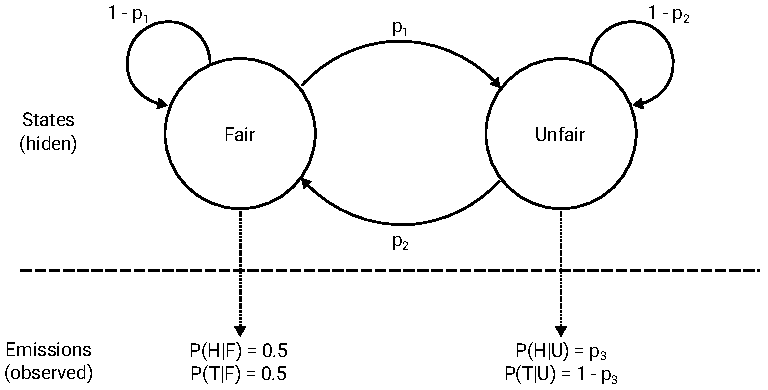
\includegraphics[width=10cm]{../report/figure1}
		\end{figure}
	\end{frame}


\end{document}